Table~\ref{tab:pathtable} reports the primary comparison on the 96
test demand paths under the frozen protocol of
Section~\ref{sec:pairresults}: flow-prediction error, attribution-column
error, family-boundary error, and the number of paths improved by
response supervision. The unrestricted and integrated-bound columns
and their group-level breakdown move to
Table~\ref{tab:boundchain96} (Appendix~\ref{supp:boundchain});
Appendix~\ref{app:pairs-v102} gives full objectives and denominators.
\begin{table}[t]\centering\footnotesize
\caption{Prediction and spatial explanation on the same 96 test demand
paths (24 per group). Entries are group medians of path-level values;
flow errors are additionally averaged over the 41 states within each
path. Family boundary: the maximum account error over the query's
boundary family, as a percentage of the reference family maximum (the
Sioux Falls family is the geometric screenline set; Anaheim uses its
ordered distance family). Improved: paths on which response supervision
lowers the error.}\label{tab:pathtable}
\setlength{\tabcolsep}{4.5pt}
\begin{tabular*}{\tblwidth}{@{\extracolsep{\fill}}rcc cc cc cc}
\toprule
& \multicolumn{2}{c}{Flow pred.\ (\%)} & \multicolumn{2}{c}{Column (\%)} & \multicolumn{2}{c}{Family boundary (\%)} & \multicolumn{2}{c}{Improved}\\
\cmidrule(lr){2-3}\cmidrule(lr){4-5}\cmidrule(lr){6-7}\cmidrule(lr){8-9}
Active & flow & resp. & flow & resp. & flow & resp. & col. & fam.\\
\midrule
1 & 0.032 & 0.029 & 8.13 & 4.92 & 2.95 & 1.78 & 24/24 & 23/24\\
2 & 0.032 & 0.029 & 21.09 & 15.67 & 8.62 & 6.19 & 22/24 & 21/24\\
3 & 0.033 & 0.029 & 21.53 & 15.46 & 9.07 & 6.01 & 22/24 & 22/24\\
6 & 0.033 & 0.030 & 22.45 & 14.22 & 9.27 & 5.77 & 24/24 & 24/24\\
\midrule
All 96 & 0.032 & 0.029 & 21.18 & 14.19 & 8.74 & 5.75 & 92/96 & 90/96\\
\bottomrule\end{tabular*}\end{table}
On the 96 test demand paths, response supervision lowers the median
attribution-column error from 21.18\% to 14.19\% (a relative reduction
of one third) and the family-boundary error from 8.74\% to 5.75\%,
while both models retain flow-prediction errors near $0.03\%$ (medians
$0.0322\%$ and $0.0292\%$). The improvement holds in every
active-query group. Path-level paired differences quantify the
uncertainty: the median paired column-error difference is $-5.03$
percentage points with a path-level bootstrap $95\%$ interval of
$[-6.01,-4.48]$ (10,000 resamples), improving 92 of 96 paths; the
paired family-boundary difference has median $-2.06$ with interval
$[-2.76,-1.65]$, improving 90 of 96, with every group's interval
excluding zero and leave-one-path-out medians varying within
$[-5.11,-4.94]$ and $[-2.11,-2.00]$
(Appendix~\ref{supp:learningdetail} reports the group-level intervals).
The system-contribution difference is secondary and opposite in sign
(median $+0.45$, interval $[0.01,0.74]$; both methods below $3.5\%$),
confirming that scalar completeness and spatial explanation accuracy
measure different properties. The same-path decomposition of
Eq.~\eqref{eq:coldecompmain} attributes the discrepancy to demand-response
error on every path--query pair (path--query median response and weight
norms $206.5$ and $3.5$ under flow supervision, $147.6$ and $3.3$ under
response supervision). Measured against the demand-change increment
rather than total flows, the endpoint flow-prediction error is
$5.1\%$ under flow supervision and $3.5\%$ under response supervision
(median of $\norm{\Delta f^L-\Delta f^S}_2/\norm{\Delta f^S}_2$ over
path--seed units; Appendix~\ref{supp:learningdetail}), so response
supervision also improves the incremental response that the
attributions decompose.

\paragraph{Six objectives under a fair weight search.}
Table~\ref{tab:fairmethods} completes the objective comparison under
the shared continuation budget and the common validation-only weight
search (Appendix~\ref{app:pairs-v102}). Each objective's auxiliary
term is normalized by a scale carrying that objective's own units ---
in particular the weighted-response term by its reference scale
$v_j^2=\langle\|D^SJ_j^S\|_2^2\rangle_j$ rather than the unweighted
scale --- so that a common weight grid explores comparable
regularization ranges; under this normalization every objective trains
at a properly selected weight. The comparison supports a family-level
conclusion. Weighted-response supervision --- the direct form
identified by the decomposition of Eq.~\eqref{eq:coldecompmain} ---
reaches a column error of $15.21\%$ at its selected weight, improves
84 of 96 paths, and trains across the whole low-to-mid weight range;
the unweighted form is the simplest member of the family and attains
the lowest errors on every metric (column $14.19\%$, family boundary
$5.75\%$, flow $0.029\%$) with the widest usable weight range,
confirming directly that the weight-shift term the unweighted
objective ignores is small. With validation-selected weights, both
endpoint objectives improve attribution accuracy relative to flow-only
training ($21.18\%\to16.2\%$ in column error), although their errors
remain above those of the response-supervised objectives. The
boundary-seminorm objective shows the largest validation--test gap:
its validation boundary error decreases monotonically with the weight
up to the selected $\lambda^*=0.3$ and reaches the lowest validation
value of any objective, yet its test column error at that weight stays
above flow-only training ($24.18\%$, improved on only 8 of 96 paths).
Optimizing the boundary value alone does not repair the underlying
response field, whereas supervising that field improves every spatial
error metric.
\begin{table}[t]\centering\footnotesize
\caption{Six supervision objectives on the same 96 test demand paths,
each at its validation-selected weight $\lambda^*$ under the shared
continuation budget and uniform selection rule
(Appendix~\ref{app:pairs-v102}); the weighted-response objective is
normalized by its own reference scale $v_j$. Entries are medians of
path-level values; improved: paths on which the objective lowers the
column (family-boundary) error relative to flow-only
training.}\label{tab:fairmethods}
\setlength{\tabcolsep}{5pt}
\begin{tabular*}{\tblwidth}{@{\extracolsep{\fill}}lcccc cc}
\toprule
Objective & $\lambda^*$ & Flow pred.\ (\%) & Column (\%) & Family boundary (\%) & \multicolumn{2}{c}{Improved vs.\ flow}\\
\cmidrule(lr){6-7}
& & & & & col. & fam.\\
\midrule
Flow only & --- & 0.032 & 21.18 & 8.74 & --- & ---\\
Response supervision & 1 & 0.029 & 14.19 & 5.75 & 92/96 & 90/96\\
Weighted response & 0.1 & 0.032 & 15.21 & 6.93 & 84/96 & 79/96\\
Boundary seminorm & 0.3 & 0.037 & 24.18 & 7.21 & 8/96 & 45/96\\
Endpoint-edge & 0.3 & 0.035 & 16.23 & 7.46 & 72/96 & 66/96\\
\quad + cut term$^{\dag}$ & 0.3 & 0.035 & 16.26 & 7.47 & 72/96 & 67/96\\
\bottomrule\end{tabular*}\end{table}
\noindent$^{\dag}$The endpoint-cut bundle is the endpoint-edge
objective plus a fixed-ratio ($0.01$) boundary term inherited from the
earlier protocol; it is reported as an ablation of that fixed mixture
ratio, not as an independently tuned competitor.
\begin{figure}[t]
\centering
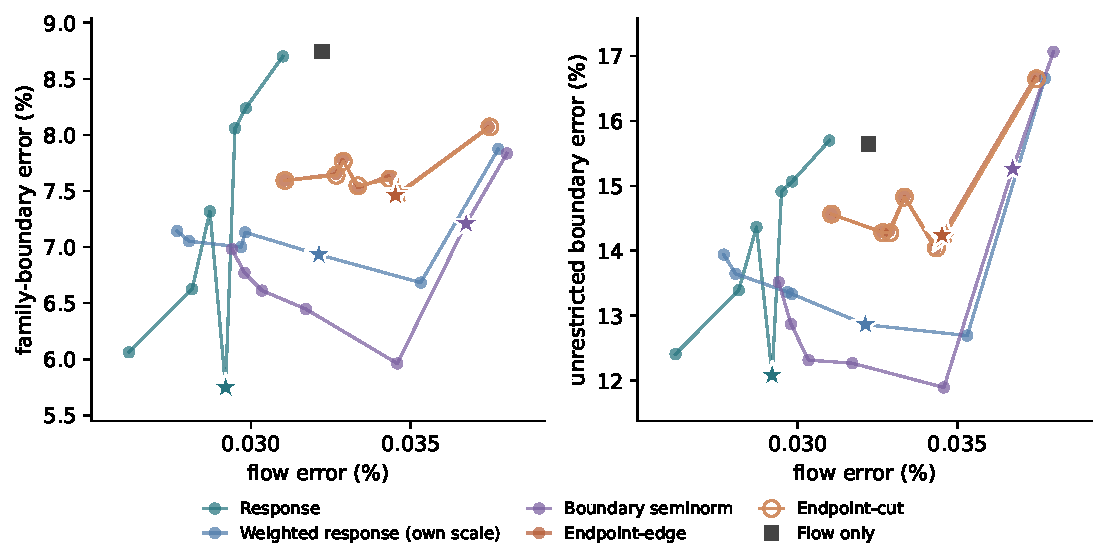
\includegraphics[width=\linewidth]{../figures/fig_v110_pareto.pdf}
\caption{Explanation--flow trade-off of the six supervision objectives
across the weight grid, on the 96 Sioux Falls test paths. Each point
is one (objective, weight) configuration: median flow error against
median family-boundary error (left) and unrestricted boundary error
(right); the validation-selected weight of each objective is starred.
Response supervision sweeps the efficient frontier in both panels,
interpolating between flow-only behaviour and the lowest boundary
error. Under its own scale normalization the weighted-response
objective tracks the same band across the low-to-mid weights; only the
largest weight fails the flow-eligibility screen and falls back to the
initial checkpoint. The boundary-seminorm objective reaches its best
errors only at unselected intermediate weights, and the endpoint
objectives (nearly coincident; the cut term is a fixed-ratio minor
addition) trace interior curves.}
\label{fig:v109pareto}
\end{figure}
The improvement is consistent across all five seeds, with both median
error metrics decreasing for every seed and 80--91 of 96 paths
improving per seed (Table~\ref{tab:fiveseed},
Appendix~\ref{supp:learningdetail}).

\paragraph{How many response labels are needed.}
Figure~\ref{fig:v109labelbudget} retrains response supervision at the
selected weight with per-query derivative-center budgets of $6$, $12$,
$24$ and $48$ (36--288 centers in total; the 64-per-query run, 384
centers, is the main comparison above), with the flow-only level drawn
for reference. A relatively small set of derivative labels recovers a
substantial fraction of the improvement obtained with the full label
set: 36 centers deliver nearly half of the full improvement over
flow-only training, and 288 centers deliver $94\%$ of it. Flow
accuracy stays within the same range at every budget (median
$0.029$--$0.033\%$, at the level of the flow-only reference line).
Each training center costs one reference flow solve and one
sensitivity solve, so response supervision is sample-efficient.
\begin{figure}[t]
\centering
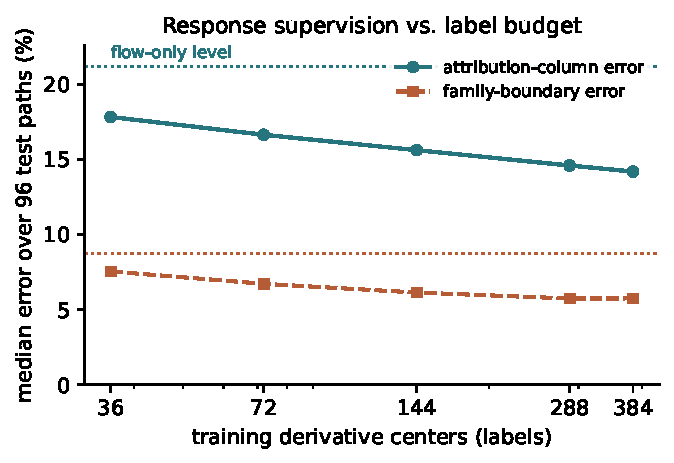
\includegraphics[width=0.72\linewidth]{../figures/fig_v110_labelbudget.pdf}
\caption{Response supervision under reduced label budgets on the 96
test paths, at the validation-selected weight: median attribution
column and family-boundary errors against the number of training
derivative centers (36--384; logarithmic axis), with the flow-only
levels marked (dotted). The full-budget point (384 centers) is the
main comparison of Table~\ref{tab:fairmethods}; flow-prediction error
stays between $0.029\%$ and $0.033\%$ at every budget and is omitted
from the axis.}\label{fig:v109labelbudget}
\end{figure}

\paragraph{Stability under a tripled training budget.}
Neither method sits at a validation plateau at the 1{,}200-update cap.
Repeating the frozen continuation protocol with the budget tripled to
3{,}600 updates (Figure~\ref{fig:v109convergence}; on Sioux Falls the
first twelve validation points --- the original 1{,}200-update budget
--- reproduce the archived runs to $10^{-12}$ in validation boundary
error) improves
both objectives on both networks, so the comparison above is not an
artifact of the cap. On the 96 test paths, flow-only training improves
its median column error from $21.18\%$ to $19.46\%$ and response
supervision from $14.19\%$ to $11.41\%$; on Anaheim's 48 paths, from
$1.64\%$ to $1.24\%$ and from $1.31\%$ to $0.88\%$. The ordering
persists and its relative margin widens on both networks (column-error
ratio $0.67\to0.59$ on Sioux Falls, $0.80\to0.71$ on Anaheim), with
flow accuracy again slightly better under response supervision.
Validation curves continue to decrease at 3{,}600 updates --- most
steeply for response supervision on Sioux Falls ($41\%$ further
boundary-error reduction from step 1{,}200) --- so the reported
operating points remain budget-limited, with the larger remaining
headroom on the response method.
\begin{figure}[t]
\centering
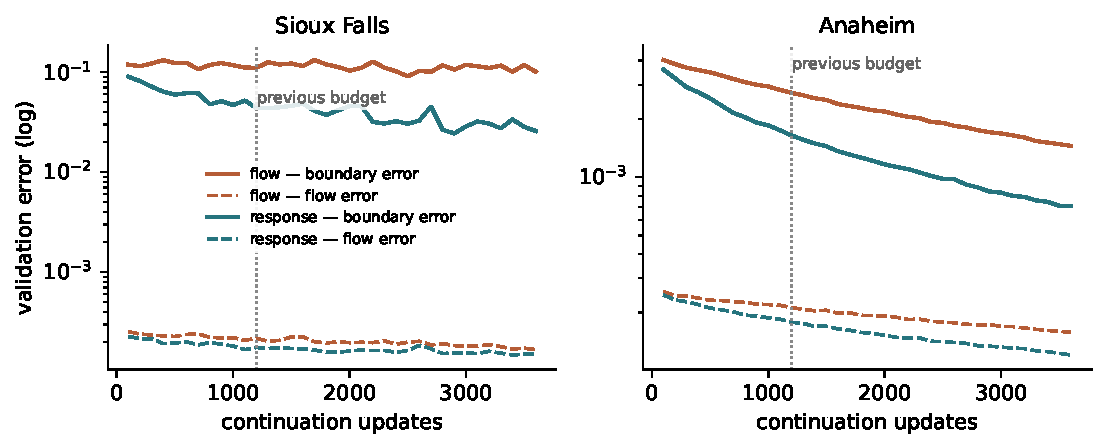
\includegraphics[width=\linewidth]{../figures/fig_v109_convergence.pdf}
\caption{Validation convergence under the tripled continuation budget
(seed-median validation boundary error, solid, and relative flow
error, dashed; log scale): Sioux Falls (left) and Anaheim (right),
flow-only (ochre) versus response supervision (teal). The dotted line
marks the previous 1{,}200-update budget; both objectives keep
improving beyond it, and the response curves stay below the
corresponding flow curves throughout.}\label{fig:v109convergence}
\end{figure}

\paragraph{Total error of the delivered summaries.}
The quantities of Table~\ref{tab:pathtable} concern the learned
profiles; the delivered artifact is the learned model's minimum-segment
summary. Table~\ref{tab:totalerror} evaluates the budget of
Eq.~\eqref{eq:totalbudget} on both networks at the working $5\%$
tolerance under a common per-query normalization (percent of the
reference family scale $\max_U|a^S_j(U)|$; the model term of
Table~\ref{tab:pathtable} reappears as $E_{\mathrm{model}}$ here).
Figure~\ref{fig:v110resolution} traces the same quantities as the
tolerance --- and with it the number of reported segments --- varies
from $0.5\%$ to $10\%$: the x axis is the number of segments a reader
must absorb, the y axis the final error of the delivered summary
against the reference explanation. The two networks occupy different
regimes, and the error budget identifies the effective lever on each.
On Sioux Falls the model term dominates ($8.74\%$ against a $4.76\%$
summary term under flow supervision), the response-supervised curve
lies strictly below the flow-supervised curve at every segment count,
and a final error of $11.5\%$ needs 77 segments under response
supervision but 117 under flow supervision --- or, at the same 117
segments, response supervision lowers the final error from $11.35\%$
to $8.68\%$. On Anaheim the learned
columns are closer to the reference, and at the working $5\%$ tolerance
the budget is compression-dominated: the summary term ($4.3\%$) is
several times the model term ($0.9\%$), the two methods deliver nearly
the same total error, and both curves track the reference-compression
curve --- the error of compressing the reference profile itself at each
tolerance, plotted at its own segment count. At the tightest $0.5\%$
tolerance the model term takes over ($0.9\%$ and $0.8\%$ against a
$0.5\%$ summary term), so tightening further there requires a better
learned response. The relative importance
of model and compression errors therefore differs across networks and
tolerances, and the error budget identifies whether improving the
learned response or
refining the spatial summary is the more effective route to a more
accurate explanation. On both networks the measured total error of the
delivered summary stays within the budget on every path. Relative to
the baselines, segmentation cuts the total error by a factor of
$3.0$--$3.8$ (single common value) and $1.7$--$2.0$ (equal-count) on
Sioux Falls, and by $10.5$--$10.6$ and $10.2$ on Anaheim --- where the
strongly ordered profiles make equal-count segmentation nearly as
coarse as a single value, so position-aware segmentation is what
carries the error control; the paired total error improves on $93.1\%$
of Sioux Falls path--query pairs under response supervision. Entries
in Table~\ref{tab:totalerror} are medians of budget components
computed on each path--query--seed before aggregation, so they do not
add to a guarantee for any single explanation.
\begin{table}[t]\centering\footnotesize
\caption{Total error budget of the learned minimum-segment summaries,
cross-network summary at tolerance $5\%$ of the learned family
maximum. Sioux Falls: 96 test paths, direction-grouped families;
Anaheim: 48 test paths, ordered families. Entries are medians of
path-level values in percent of the reference family scale
($\max_U|a^S_j(U)|$), computed per path--query--seed and averaged
within path; Sioux Falls segments are summed over the family's
distinct direction chains (duplicate projection directions removed).
Single: one common value for the whole family; equal: equal-count
segmentation with the same per-direction
counts.}\label{tab:totalerror}
\setlength{\tabcolsep}{4.5pt}
\begin{tabular*}{\tblwidth}{@{\extracolsep{\fill}}llcccccc}
\toprule
Network & Method & $E_{\mathrm{model}}$ & $E_{\mathrm{summary}}$ & $E_{\mathrm{total}}$ & Single & Equal & Segments\\
\midrule
Sioux Falls & Flow & 8.74 & 4.76 & 11.35 & 34.3 & 19.7 & 117\\
Sioux Falls & Response & 5.75 & 4.75 & 8.68 & 33.0 & 17.2 & 117\\
\addlinespace
Anaheim & Flow & 0.94 & 4.33 & 4.57 & 48.0 & 46.6 & 9.9\\
Anaheim & Response & 0.78 & 4.32 & 4.55 & 48.0 & 46.6 & 9.9\\
\bottomrule\end{tabular*}\end{table}
\begin{figure}[t]
\centering
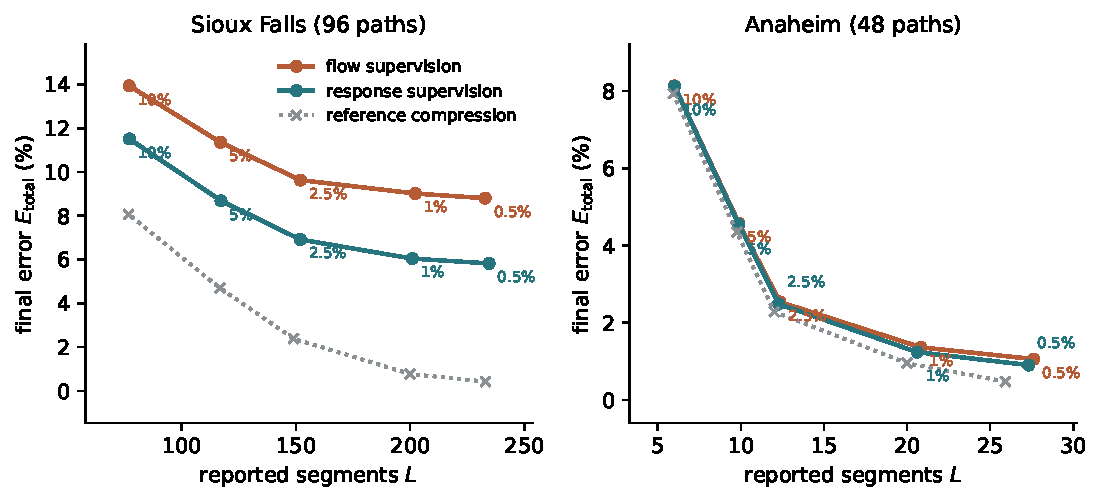
\includegraphics[width=\linewidth]{../figures/fig_v110_resolution.pdf}
\caption{Final error of the delivered summary against the number of
reported segments, as the family tolerance varies over
$0.5$--$10\%$ (annotated; percent of the learned family maximum).
Sioux Falls (left): model-error dominated --- the response-supervised
curve (teal) lies below the flow-supervised curve (ochre) at every
segment count, so better responses convert into either fewer segments
at equal accuracy or more accurate summaries at equal complexity.
Anaheim (right): compression dominated at the working tolerance ---
both curves track the grey reference-compression curve, the error of
compressing the reference profile itself at each tolerance, plotted at
its own segment count ($\times$ marks). Per-tolerance segmentation
recomputed from the frozen learned profiles; common per-query
normalization as in
Table~\ref{tab:totalerror}.}\label{fig:v110resolution}
\end{figure}

\paragraph{Bound tightness.}
Computed with the same $41$-state trapezoidal quadrature for both
sides, the exact unrestricted errors $\mathcal K_j(e_j)$ lie below the
integrated bounds $B_j$ of Eq.~\eqref{eq:localboundarybound} (the
numerical verification and quadrature accuracy are reported in
Appendix~\ref{supp:accuracy}). The chain is tight: the median ratio
$\mathcal K_j(e_j)/B_j$ is $0.95$ for flow supervision (quartiles
$0.91$--$0.98$) and $0.95$ for response supervision (quartiles
$0.90$--$0.97$). The integrated bound is therefore a tight
\emph{a posteriori} upper bound on the realized worst boundary error
--- it uses reference-response information, as
Section~\ref{sec:totalbudget} notes --- and response supervision lowers
the family, unrestricted and bound levels in parallel. The geometric
family retains about half of the unrestricted error (median
ratio $E^{\mathrm{geo}}/\mathcal K_j(e_j)$ $0.51$ and $0.48$), so the
single-family errors reported throughout should be read as lower
bounds on the worst separating-region error. Sign reliability on the
separate frozen six-query baseline segment is boundary specific and is
retained in Appendix~\ref{supp:screenlinelearned}.
